\begin{figure}[tb]
    \centering
    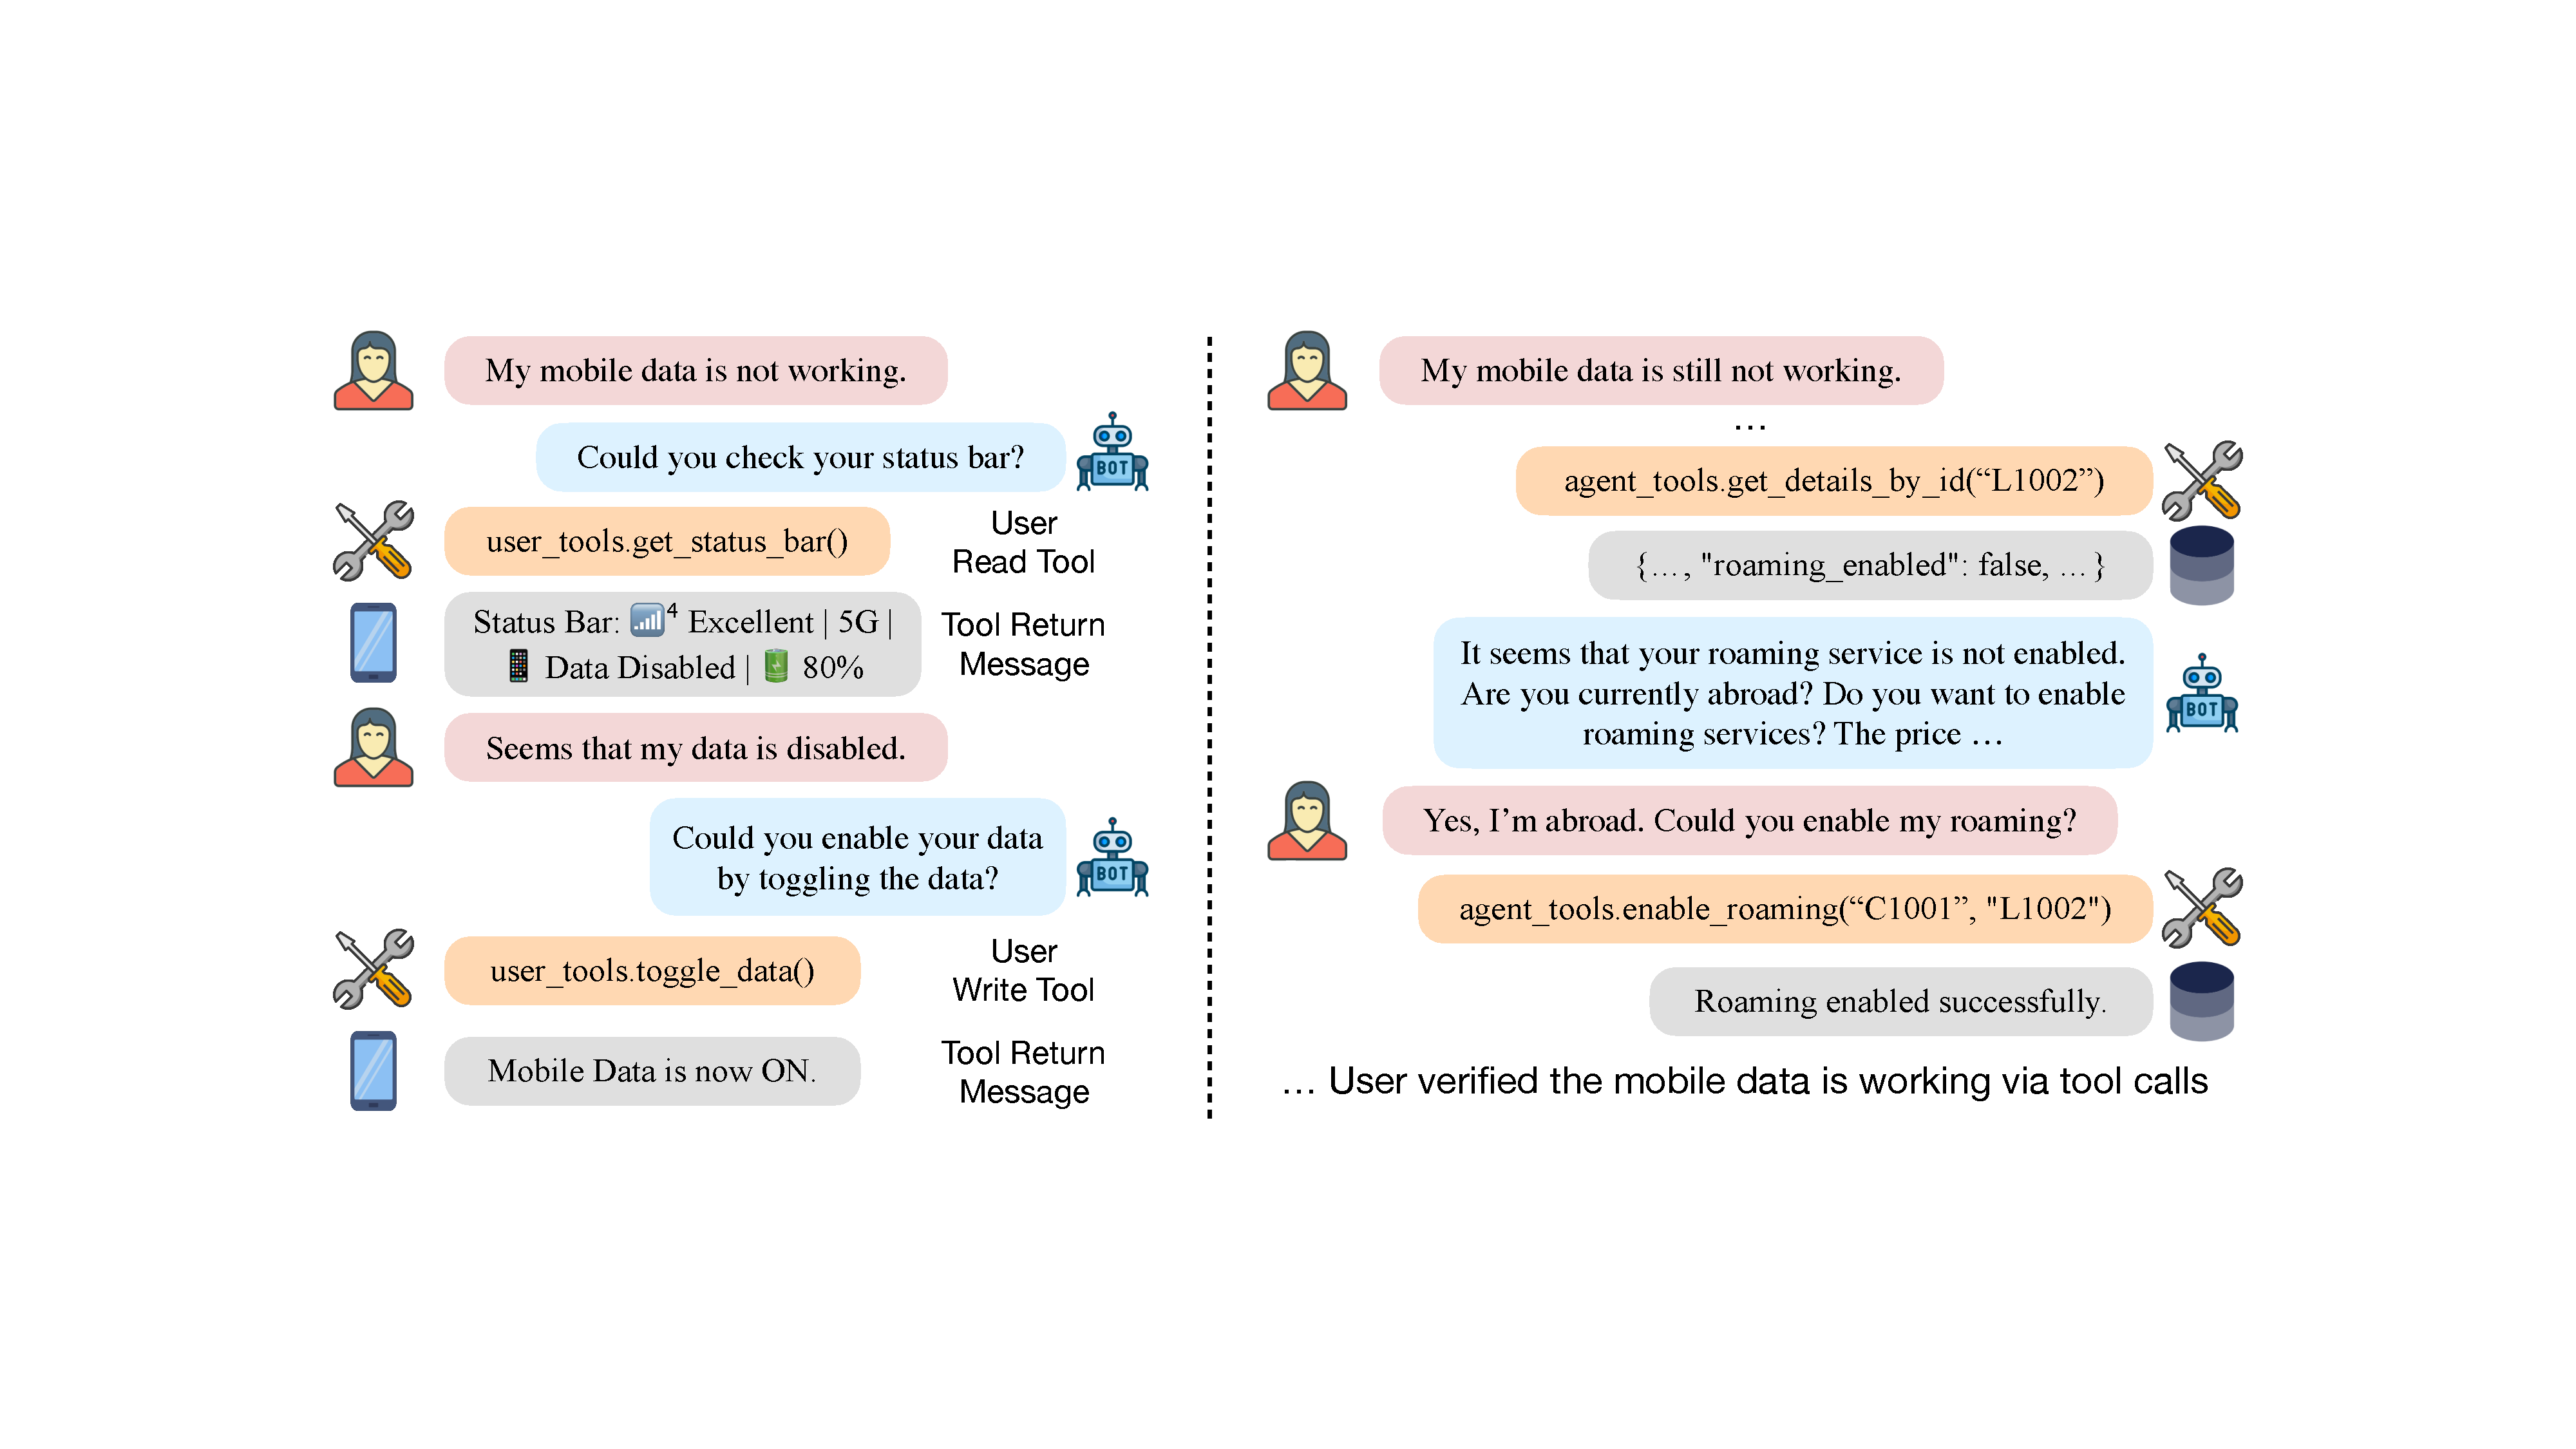
\includegraphics[width=0.99\textwidth,trim=240 240 240 240,clip]{figures/raw/traj.pdf}
    \vspace{-0.5em}
    \caption{\telecom 도메인에서 \bench의 에이전트-사용자 상호작용 trajectory($\gS_{history}$) 예시. 사용자 도구(모의 전화)의 구현을 제어함으로써, 기저 데이터베이스 상태를 바탕으로 ``상태 표시줄 확인''과 ``데이터 전환'' 같은 에이전트의 실행 가능한 지시에 대한 사용자의 응답을 안정적으로 시뮬레이션할 수 있다. 오른쪽 절반에서는 에이전트의 도구 호출이 사용자의 데이터베이스 상태에 미치는 영향을 모델링할 수 있음을 보여 주며, 여기서는 사용자에 대한 roaming 서비스가 에이전트 쪽에서 활성화되어 사용자의 전화가 roaming할 수 있게 된다.}
    \label{fig:traj}
\end{figure}
